% Ce fichier main.tex est le fichier principal \`{a} partir duquel tout est g\'{e}n\'{e}r\'{e}
% This file is the main file where the final document is generated
\documentclass{these-dbl}

% Remplir les metadonnees du pdf
% Fill the pdf metadata
\hypersetup{
%    pdfauthor   = {XYZ},
%    pdftitle    = {Th\`{e}se de doctorat de XYZ},
%    pdfsubject  = {Th\`{e}se de doctorat de XYZ},
%    pdfkeywords = {mots-cl\'{e}s},
}

\geometry{vmargin=4.0cm}

% Spécifier vos fichiers de bibliographie
% Specify you bibliography files here
\addbibresource{./biblio/biblio.bib}

\begin{document}

% Page de garde avec commande \maketitle
% Front cover calling \maketitle
% La page de garde est en français
% The front cover is in French
\selectlanguage{french}

% Inclure les infos de chaque établissement
% Include each institution data

%%% Switch case in latex
%%% https://tex.stackexchange.com/a/343306
\makeatletter
\newcommand\addcase[3]{\expandafter\def\csname\string#1@case@#2\endcsname{#3}}
\newcommand\makeswitch[2][]{%
  \newcommand#2[1]{%
    \ifcsname\string#2@case@##1\endcsname\csname\string#2@case@##1\endcsname\else#1\fi%
  }%
}
\makeatother

%%%% Il faut adapter la taille des logos dans certains cas (e.g., EGAAL, 2 etablissements)
\newcommand\hauteurlogos[3]{
    \hauteurlogoecole{#1}
    \hauteurlogoetablissementA{#2}
    \hauteurlogoetablissementB{#3}
}

%%%%%%%%%%%%%%%%%%%%%%%%%%%%%%%%%%%%%%%%%%%%%%%%%%%
%%%%%%%%%%%%%%%% ECOLES DOCTORALES %%%%%%%%%%%%%%%%

%%%% #1: dossier des images, #2: numero ED, #3: couleur ED, #4-#5: nom complet sur plusieurs lignes
\newcommand\addecoledoctorale[5]{\direcole{#1}\numeroecole{#2}\definecolor{color-ecole}{RGB}{#3}\nomecoleA{#4}\nomecoleB{#5}}

\makeswitch[default]\ecoledoctorale{}

\addcase\ecoledoctorale{MaSTIC}{\addecoledoctorale
    {MaSTIC} %nom du dossier où sont les images
    {641} %numéro ed
    {109,65,207} %code couleur
    {Math\'{e}matiques et Sciences et Technologies du numérique,}
    {de l’Information et de la Communication} }


\addcase\ecoledoctorale{3M}{\addecoledoctorale
    {3M}
    {596}
    {193,192,183}
    {Mati\`{e}re, Mol\'{e}cules, Mat\'{e}riaux}
    {}
}
\addcase\ecoledoctorale{ALL}{\addecoledoctorale
    {ALL}
    {595}
    {240,209,134}
    {Arts, Lettres, Langues}
    {}
}
\addcase\ecoledoctorale{BS}{\addecoledoctorale
    {BS}
    {605}
    {163,219,208}
    {Biologie, Sant\'{e}}
    {}
}
\addcase\ecoledoctorale{DSP}{\addecoledoctorale
    {DSP}
    {599}
    {188,208,220}
    {Droit et Science politique}
    {}
}
\addcase\ecoledoctorale{EDGE}{\addecoledoctorale
    {EDGE}
    {597}
    {216,178,210}
    {Sciences \'{E}conomiques et sciences De Gestion}
    {}
}
\addcase\ecoledoctorale{EGAAL}{\addecoledoctorale
    {EGAAL}
    {600}
    {146,213,182}
    {\'{E}cologie, G\'{e}osciences, Agronomie et Alimentation}
    {}
    \hauteurlogos{2cm}{2cm}{2cm}
}
\addcase\ecoledoctorale{ELICC}{\addecoledoctorale
    {ELICC}
    {603}
    {249,201,188}
    {\'{E}ducation, Langages, Interactions, Cognition, Clinique}
    {}
    \hauteurlogos{2cm}{2cm}{2cm}
}
\addcase\ecoledoctorale{MathSTIC}{\addecoledoctorale
    {MathSTIC}
    {641}
    {109,65,207} %{236,115,127}
    {Math\'{e}matiques et Sciences et Technologies du num\'{e}rique}
    {de l'Information et de la Communication}
}
\addcase\ecoledoctorale{SML}{\addecoledoctorale
    {SML}
    {598}
    {162,225,230}
    {Sciences de la Mer et du Littoral}
    {}
}
\addcase\ecoledoctorale{SPI}{\addecoledoctorale
    {SPI}
    {602}
    {159,182,217}
    {Sciences pour l'Ing\'{e}nieur}
    {}
}
\addcase\ecoledoctorale{STT}{\addecoledoctorale
    {STT}
    {604}
    {172,184,192}
    {Soci\'{e}t\'{e}s, temps, territoires}
    {}
}



%%%%%%%%%%%%%%%%%%%%%%%%%%%%%%%%%%%%%%%%%%%%%%%%
%%%%%%%%%%%%%%%% ETABLISSEMENTS %%%%%%%%%%%%%%%%

%%%% #1 nom du logo, #2-#4: nom complet sur plusieurs lignes
\newcommand\addetablissement[4]{\logoetablissementB{#1}\nometablissementC{#2}\nometablissementD{#3}\nometablissementE{#4}}

\makeswitch[default]\etablissement{}

\addcase\etablissement{CS}{\addetablissement
    {CS}
    {}
    {}
    {CENTRALESUP\'{E}LEC}
}
\addcase\etablissement{ECN}{\addetablissement
    {ECN}
    {}
    {}
    {L'\'{E}COLE CENTRALE DE NANTES}
}
\addcase\etablissement{EHESP}{\addetablissement
    {EHESP}
    {}
    {L'\'{E}COLE DES HAUTES \'{E}TUDES}
    {EN SANT\'{E} PUBLIQUE DE RENNES}
}
\addcase\etablissement{ENIB}{\addetablissement
    {ENIB}
    {}
    {L'\'{E}COLE NATIONALE}
    {D'ING\'{E}NIEURS DE BREST}
}
\addcase\etablissement{ENS}{\addetablissement
    {ENS}
    {}
    {L'\'{E}COLE NORMALE}
    {SUP\'{E}RIEURE RENNES}
}
\addcase\etablissement{ENSA}{\addetablissement
    {ENSA}
    {}
    {L'\'{E}COLE NORMALE SUP\'{E}RIEURE}
    {D'ARCHITECTURE DE NANTES}
}
\addcase\etablissement{ENSAB}{\addetablissement
    {ENSAB}
    {}
    {L'\'{E}COLE NORMALE SUP\'{E}RIEURE}
    {D'ARCHITECTURE DE BRETAGNE}
}
\addcase\etablissement{ENSAI}{\addetablissement
    {ENSAI}
    {}
    {L'\'{E}COLE NATIONALE DE LA STATISTIQUE}
    {ET DE L'ANALYSE DE L'INFORMATION}
}
\addcase\etablissement{ENSCR}{\addetablissement
    {ENSCR}
    {}
    {L'\'{E}COLE NATIONALE SUP\'{E}RIEURE}
    {DE CHIMIE RENNES}
}
\addcase\etablissement{ENSTA}{\addetablissement
    {ENSTA}
    {}
    {L'\'{E}COLE NATIONALE SUP\'{E}RIEURE}
    {DE TECHNIQUES AVANC\'{E}ES BRETAGNE}
}
\addcase\etablissement{IMTA}{\addetablissement
    {IMTA}
    {L'\'{E}COLE NATIONALE SUP\'{E}RIEURE}
    {MINES-T\'{E}L\'{E}COM ATLANTIQUE BRETAGNE}
    {PAYS-DE-LA-LOIRE - IMT ATLANTIQUE}
}
\addcase\etablissement{INSA}{\addetablissement
    {INSA}
    {}
    {L'INSTITUT NATIONAL DES}
    {SCIENCES APPLIQU\'{E}ES RENNES}
}
\addcase\etablissement{InstitutAgro}{\addetablissement
    {InstitutAgro}
    {L'INSTITUT NATIONAL D'ENSEIGNEMENT SUP\'{E}RIEUR}
    {POUR L'AGRICULTURE, L'ALIMENTATION ET}
    {L'ENVIRONNEMENT - ECOLE INTERNE AGROCAMPUS OUEST}
}
\addcase\etablissement{LMU}{\addetablissement
    {LMU}
    {}
    {}
    {LE MANS UNIVERSIT\'{E}}
}
\addcase\etablissement{Oniris}{\addetablissement
    {Oniris}
    {}
    {}
    {ONIRIS}
}
\addcase\etablissement{UA}{\addetablissement
    {UA-couleur}
    {}
    {}
    {L'UNIVERSIT\'{E} D'ANGERS}
}
\addcase\etablissement{UB}{\addetablissement
    {UB}
    {}
    {}
    {L'UNIVERSIT\'{E} DE BREST}
}
\addcase\etablissement{UBO}{\addetablissement
    {UBO}
    {}
    {}
    {L'UNIVERSIT\'{E} DE BRETAGNE OCCIDENTALE}
}
\addcase\etablissement{UBS}{\addetablissement
    {UBS}
    {}
    {}
    {L'UNIVERSIT\'{E} DE BRETAGNE SUD}
}
\addcase\etablissement{UN}{\addetablissement
    {UN-noir}
    {}
    {}
    {NANTES UNIVERSIT\'{E}}
}
\addcase\etablissement{UR1}{\addetablissement
    {UR1-noir}
    {}
    {}
    {L'UNIVERSIT\'{E} DE RENNES 1}
}
\addcase\etablissement{UR2}{\addetablissement
    {UR2}
    {}
    {}
    {L'UNIVERSIT\'{E} DE RENNES 2}
}


%%%% #1-#2: nom des deux logos, #3-#7: nom complet de la double affiliation sur plusieurs lignes
\newcommand\addpairetablissements[7]{
    \logoetablissementA{#1}
    \logoetablissementB{#2}
    \nometablissementA{#3}
    \nometablissementB{#4}
    \nometablissementC{#5}
    \nometablissementD{#6}
    \nometablissementE{#7}
}

% ALL, STT: UR2-ENSAB
\addcase\etablissement{UR2-ENSAB}{\addpairetablissements
    {ENSAB}
    {UR2}
    {}
    {L'\'{E}COLE NORMALE SUP\'{E}RIEURE}
    {D'ARCHITECTURE DE BRETAGNE}
    {D\'{E}LIVR\'{E}E CONJOINTEMENT AVEC}
    {L'UNIVERSIT\'{E} DE RENNES 2}
    \hauteurlogos{2cm}{1.2cm}{2cm}
}
% BS, DSP, MathSTIC: UR1-UR2
\addcase\etablissement{UR1-UR2}{\addpairetablissements
    {UR2}
    {UR1-noir}
    {}
    {}
    {L'UNIVERSIT\'{E} DE RENNES 2}
    {D\'{E}LIVR\'{E}E CONJOINTEMENT AVEC}
    {L'UNIVERSIT\'{E} DE RENNES 1}
    \hauteurlogos{2cm}{2cm}{2cm}
}
% DSP, EDGE: UR1-EHESP
\addcase\etablissement{UR1-EHESP}{\addpairetablissements
    {EHESP}
    {UR1-noir}
    {}
    {L'UNIVERSIT\'{E} DE RENNES 1}
    {D\'{E}LIVR\'{E}E CONJOINTEMENT AVEC}
    {L'\'{E}COLE DES HAUTES \'{E}TUDES}
    {EN SANT\'{E} PUBLIQUE DE RENNES}
    \hauteurlogos{2cm}{2cm}{2cm}
}
% EGAAL: UA-LMU
\addcase\etablissement{UA-LMU}{\addpairetablissements
    {LMU}
    {UA-couleur}
    {}
    {}
    {LE MANS UNIVERSIT\'{E}}
    {D\'{E}LIVR\'{E}E CONJOINTEMENT AVEC}
    {L'UNIVERSIT\'{E} D'ANGERS}
    \hauteurlogos{2cm}{1cm}{2cm}
}
% MathSTIC: UR1-InstitutAgro
\addcase\etablissement{UR1-InstitutAgro}{\addpairetablissements
    {InstitutAgro}
    {UR1-noir}
    {L'INSTITUT NATIONAL D'ENSEIGNEMENT SUP\'{E}RIEUR}
    {POUR L'AGRICULTURE, L'ALIMENTATION ET}
    {L'ENVIRONNEMENT - ECOLE INTERNE AGROCAMPUS OUEST}
    {D\'{E}LIVR\'{E}E CONJOINTEMENT AVEC}
    {L'UNIVERSIT\'{E} DE RENNES 1}
    \hauteurlogos{1.8cm}{1.3cm}{1.5cm}
}
% SML: UBO-IMTA
\addcase\etablissement{UBO-IMTA}{\addpairetablissements
    {IMTA}
    {UBO}
    {L'\'{E}COLE NATIONALE SUP\'{E}RIEURE}
    {MINES-T\'{E}L\'{E}COM ATLANTIQUE BRETAGNE}
    {PAYS-DE-LA-LOIRE - IMT ATLANTIQUE}
    {D\'{E}LIVR\'{E}E CONJOINTEMENT AVEC}
    {L'UNIVERSIT\'{E} DE BRETAGNE OCCIDENTALE}
    \hauteurlogos{2cm}{1.8cm}{1.8cm}
}
% SPI: ECN-ENSA
\addcase\etablissement{ECN-ENSA}{\addpairetablissements
    {ENSA}
    {ECN}
    {}
    {L'\'{E}COLE NORMALE SUP\'{E}RIEURE}
    {D'ARCHITECTURE DE NANTES}
    {D\'{E}LIVR\'{E}E CONJOINTEMENT AVEC}
    {L'\'{E}COLE CENTRALE DE NANTES}
    \hauteurlogos{2cm}{1.8cm}{1.8cm}
}
% SPI: UBO-ENIB
\addcase\etablissement{UBO-ENIB}{\addpairetablissements
    {ENIB}
    {UBO}
    {}
    {L'\'{E}COLE NATIONALE}
    {D'ING\'{E}NIEURS DE BREST}
    {D\'{E}LIVR\'{E}E CONJOINTEMENT AVEC}
    {L'UNIVERSIT\'{E} DE BRETAGNE OCCIDENTALE}
    \hauteurlogos{2cm}{1.8cm}{1.6cm}
}
% SPI: UN-Oniris
\addcase\etablissement{UN-Oniris}{\addpairetablissements
    {Oniris}
    {UN-noir}
    {}
    {}
    {ONIRIS}
    {D\'{E}LIVR\'{E}E CONJOINTEMENT AVEC}
    {L'UNIVERSIT\'{E} DE NANTES}
    \hauteurlogos{2cm}{2cm}{2cm}
}
% STT: ENSA-UN
\addcase\etablissement{ENSA-UN}{\addpairetablissements
    {ENSA}
    {UN-noir}
    {}
    {L'\'{E}COLE NORMALE SUP\'{E}RIEURE}
    {D'ARCHITECTURE DE NANTES}
    {D\'{E}LIVR\'{E}E CONJOINTEMENT AVEC}
    {L'UNIVERSIT\'{E} DE NANTES}
    \hauteurlogos{2cm}{2cm}{2cm}
}


% Inclure infos de l'école doctorale
% Include doctoral school data
% (3M ALL BS DSP EDGE EGAAL ELICC MathSTIC SML SPI STT)
\ecoledoctorale{MathSTIC}

% Inclure infos de l'établissement
% Include institution data
\etablissement{UN}

%Inscrivez ici votre sp\'{e}cialit\'{e} (voir liste des sp\'{e}cialit\'{e}s sur le site de votre \'{e}cole doctorale)
%Indicate the domain (see list of domains in your ecole doctorale)
\spec{« voir liste sur le site de votre \'{e}cole doctorale -- Informatique »}

%Attention : le pr\'{e}nom doit être en minuscules (Jean) et le NOM en majuscules (BRITTEF) 
%Attention : the first name in small letters and the name in Capital letters 
\author{« Pr\'{e}nom NOM »}

% Donner le titre complet de la th\`{e}se, \'{e}ventuellement le sous titre, si n\'{e}cessaire sur plusieurs lignes 
%Give the complete title of the thesis, if necessary on several lines
\title{« Titre de la th\`{e}se »}
\lesoustitre{« Sous-titre de la th\`{e}se »}

%Indiquer la date et le lieu de soutenance de la th\`{e}se 
%indicates the date and the place of the defense 
\date{« date »}
\lieu{« Lieu »}

%Indiquer le nom du (ou des) laboratoire (s) dans le(s)quel(s) le travail de th\`{e}se a \'{e}t\'{e} effectu\'{e}, indiquer aussi si souhait\'{e} le nom de la (les) facult\'{e}(s) (UFR, \'{e}cole(s), Institut(s), Centre(s)...), son (leurs) adresse(s)... 
%Indicates the name (or names) of research laboratories where the work has been done as well as (if desired) the names of faculties (UFR, Schools, institution...
\uniterecherche{« voir liste sur le site de votre \'{e}cole doctorale - umr6004 – LS2N»}

%Indiquer le Numero de th\`{e}se, si cela est opportun, ou laisser vide pour faire disparaitre cet ligne de la couverture
%Indicate the number of the thesis if there is one. otherwise leave empty so the line disappeurs on the cover
\numthese{« si pertinent »} % \numthese{}

%Indiquer le Pr\'{e}nom en minuscules et le Nom en majuscules, le titre de la personne et l’\'{e}tablissement dans lequel il effectue sa recherche  
%Indicates the first name on small letters and the Names on capital letters, the person's title and the institution where he/she belongs to.
%Exemples :  Examples :
%%%- Professeur, Universit\'{e} d’Angers 
%%%- Chercheur, CNRS, \'{e}cole Centrale de Nantes 
%%%-  Professeur d’universit\'{e} – Praticien Hospitalier, Universit\'{e} Paris V  
%%%-  Maitre de conf\'{e}rences, Oniris 
%%%- Charg\'{e} de recherche, INSERM, HDR, Universit\'{e} de Tours  
 %S’il n’y a pas de co-direction, faire disparaitre cet item de la couverture  
 %In there is no co-director, remove the item from the cover
\jury{
{\normalTwelve \textbf{Rapporteurs avant soutenance :}}\\ \newline
\footnotesizeTwelve
\begin{tabular}{@{}ll}
Pr\'{e}nom NOM & Fonction et \'{e}tablissement d'exercice \\
Pr\'{e}nom NOM & Fonction et \'{e}tablissement d'exercice \\
Pr\'{e}nom NOM & Fonction et \'{e}tablissement d'exercice \\
\end{tabular}

\vspace{\baselineskip}
{\normalTwelve \textbf{Composition du Jury :}}\\
{\fontsize{9.5}{11}\selectfont {\textcolor{red}{\textit{Attention, en cas d’absence d’un des membres du Jury le jour de la soutenance, la composition du jury doit être revue pour s’assurer qu’elle est conforme et devra être répercutée sur la couverture de thèse}}}}\\ \newline
\footnotesizeTwelve
\begin{tabular}{@{}lll}

Pr\'{e}sident :        & Pr\'{e}nom NOM & Fonction et \'{e}tablissement d'exercice \textit{(à préciser après la soutenance)} \\
Examinateurs :         & Pr\'{e}nom NOM & Fonction et \'{e}tablissement d'exercice \\
                       & Pr\'{e}nom NOM & Fonction et \'{e}tablissement d'exercice \\
                       & Pr\'{e}nom NOM & Fonction et \'{e}tablissement d'exercice \\
                       & Pr\'{e}nom NOM & Fonction et \'{e}tablissement d'exercice \\
Dir. de th\`{e}se :    & Pr\'{e}nom NOM & Fonction et \'{e}tablissement d'exercice \\
Co-dir. de th\`{e}se : & Pr\'{e}nom NOM & Fonction et \'{e}tablissement d'exercice \textit{(si pertinent)} \\
\end{tabular}

\vspace{\baselineskip}
{\normalTwelve \textbf{Invit\'{e}(s) :}}\\ \newline
\footnotesizeTwelve
\begin{tabular}{@{}ll}
Pr\'{e}nom NOM & Fonction et \'{e}tablissement d'exercice \\
\end{tabular}
}


\maketitle


% Sélectionner la langue du contenu suivant cette ligne
% Select the content language following this line
\selectlanguage{french}

% Inclusion du chapitre remerciement
% Input acknowledgement chapter
\clearemptydoublepage
\chapter*{Acknowledgement}

Je tiens à remercier  \\
I would like to thank. my parents..\\
J'adresse également toute ma reconnaissance à .... \\
....


% Ne pas oublier cette commande qui g\'{e}n\`{e}re la page de couverture avant
% This command will generate the front cover
\frontmatter
\clearemptydoublepage
\renewcommand{\contentsname}{Table of Contents}
\tableofcontents %sommaire %table of content
%\shorttableofcontents{Sommaire}{0}

\clearemptydoublepage
\chapter*{Introduction}
\addcontentsline{toc}{chapter}{Introduction}
\chaptermark{Introduction}


Lorem ipsum dolor sit amet, «~consectetuer~» adipiscing elit. Maecenas fermentum, elit non lobortis cursus, orci velit suscipit est, id mollis turpis mi eget orci. Ut aliquam sollicitudin metus. Mauris at sapien sed sapien congue iaculis. Nulla lorem urna, bibendum id, laoreet iaculis, nonummy eget, massa. Phasellus ullamcorper commodo velit. Class aptent taciti sociosqu ad litora torquent per «~conubia nostra~», per inceptos hymenaeos. Phasellus est. Maecenas felis augue, gravida quis, porta adipiscing, iaculis vitae, felis. Nullam ipsum. Nulla a sem ac leo fringilla mattis. Phasellus egestas augue in sem. Etiam ac enim non mauris ullamcorper scelerisque. In wisi leo, malesuada vulputate, tempor sit amet, facilisis vel, velit. Mauris massa est, sodales placerat, luctus id, hendrerit a, urna. Nullam eleifend pede eget odio. Duis non erat. Nullam pellentesque.

\begin{verse}
Maître Corbeau, sur un arbre perché, \\
Tenait en son bec un fromage. \\
Maître Renard, par l'odeur alléché, \\
Lui tint à peu près ce langage : \\
«~Hé ! bonjour, Monsieur du Corbeau. \\
Que vous êtes joli ! que vous me semblez beau ! \\
Sans mentir, si votre ramage \\
Se rapporte à votre plumage, \\
Vous êtes le Phénix des hôtes de ces bois.~» \\
\end{verse}

Lorem ipsum dolor sit amet, consectetuer adipiscing elit. Maecenas fermentum, elit non lobortis cursus, orci velit suscipit est, id mollis turpis mi eget orci. Ut aliquam sollicitudin metus. Mauris at sapien sed sapien congue iaculis. Nulla lorem urna, bibendum id, laoreet iaculis, nonummy eget, massa\footcite[32]{Pierre1901}. Phasellus ullamcorper commodo velit. Class aptent taciti sociosqu ad litora torquent per conubia nostra, per inceptos hymenaeos. Phasellus est. Maecenas felis augue, gravida quis, porta adipiscing, iaculis vitae, felis. Nullam ipsum. Nulla a sem ac leo fringilla mattis. Phasellus egestas augue in sem. Etiam ac enim non mauris ullamcorper scelerisque. In wisi leo, malesuada vulputate, tempor sit amet, facilisis vel, velit. Mauris massa est, sodales placerat, luctus id, hendrerit a, urna. Nullam eleifend pede eget odio. Duis non erat. Nullam pellentesque. 

\section*{Première section de l'intro}
\addcontentsline{toc}{section}{Première section de l'intro}

Lorem ipsum dolor sit amet, «~consectetuer~» adipiscing elit. Maecenas fermentum, elit non lobortis cursus, orci velit suscipit est, id mollis turpis mi eget orci. Ut aliquam sollicitudin metus. Mauris at sapien sed sapien congue iaculis. Nulla lorem urna, bibendum id, laoreet iaculis, nonummy eget, massa. Phasellus ullamcorper commodo velit. Class aptent taciti sociosqu ad litora torquent per «~conubia nostra~», per inceptos hymenaeos. Phasellus est. Maecenas felis augue, gravida quis, porta adipiscing, iaculis vitae, felis. Nullam ipsum. Nulla a sem ac leo fringilla mattis. Phasellus egestas augue in sem. Etiam ac enim non mauris ullamcorper scelerisque. In wisi leo, malesuada vulputate, tempor sit amet, facilisis vel, velit. Mauris massa est, sodales placerat, luctus id, hendrerit a, urna. Nullam eleifend pede eget odio. Duis non erat. Nullam pellentesque.

\textbf{Une boite magique : }

\boitemagique{Titre de la boite}{
Praesent placerat, ante at venenatis pretium, diam turpis faucibus arcu, nec vehicula quam lorem ut leo. Sed facilisis, augue in pharetra dapibus, ligula justo accumsan massa, eu suscipit felis ipsum eget enim.
}

Laoreet iaculis, nonummy eget, massa. Phasellus ullamcorper commodo velit. Class aptent taciti sociosqu ad litora torquent per «~conubia nostra~», per inceptos hymenaeos. Phasellus est. Maecenas felis augue, gravida quis, porta adipiscing, iaculis vitae, felis. Nullam ipsum. Nulla a sem ac leo fringilla mattis. Phasellus egestas augue in sem. Etiam ac enim non mauris ullamcorper scelerisque. In wisi leo, malesuada vulputate, tempor sit amet, facilisis vel, velit. Mauris massa est, sodales placerat, luctus id, hendrerit a, urna. Nullam eleifend pede eget odio. Duis non erat. Nullam pellentesque.

\textbf{Une boite simple : }
\boitesimple{Mauris lorem quam, tristique sollicitudin egestas sed, sodales vel leo. In hac habitasse platea dictumst. Lorem ipsum dolor sit amet, consectetur adipiscing elit. Sed sed lorem lacus, at venenatis elit. Pellentesque nisl arcu, blandit ac eleifend non, sodales a quam.}

Laoreet iaculis, nonummy eget, massa. Phasellus ullamcorper commodo velit. Class aptent taciti sociosqu ad litora torquent per «~conubia nostra~», per inceptos hymenaeos. Phasellus est. Maecenas felis augue, gravida quis, porta adipiscing, iaculis vitae, felis. Nullam ipsum. Nulla a sem ac leo fringilla mattis. Phasellus egestas augue in sem. Etiam ac enim non mauris ullamcorper scelerisque. In wisi leo, malesuada vulputate, tempor sit amet, facilisis vel, velit. Mauris massa est, sodales placerat, luctus id, hendrerit a, urna. Nullam eleifend pede eget odio. Duis non erat. Nullam pellentesque.




\clearemptydoublepage
\mainmatter

\clearemptydoublepage
\chapter{Titre du premier chapitre}

Lorem ipsum dolor sit amet, «~consectetuer~» adipiscing elit. Maecenas fermentum, elit non lobortis cursus, orci velit suscipit est, id mollis turpis mi eget orci. Ut aliquam sollicitudin metus. Mauris at sapien sed sapien congue iaculis. Nulla lorem urna, bibendum id, laoreet iaculis, nonummy eget, massa. Phasellus ullamcorper commodo velit. Class aptent taciti sociosqu ad litora torquent per «~conubia nostra~», per inceptos hymenaeos. Phasellus est. Maecenas felis augue, gravida quis, porta adipiscing, iaculis vitae, felis. Nullam ipsum. Nulla a sem ac leo fringilla mattis. Phasellus egestas augue in sem. Etiam ac enim non mauris ullamcorper scelerisque. In wisi leo, malesuada vulputate, tempor sit amet, facilisis vel, velit. Mauris massa est, sodales placerat, luctus id, hendrerit a, urna. Nullam eleifend pede eget odio. Duis non erat. Nullam pellentesque.

Lorem ipsum dolor sit amet, consectetuer adipiscing elit. Maecenas fermentum, elit non lobortis cursus, orci velit suscipit est, id mollis turpis mi eget orci. Ut aliquam sollicitudin metus. Mauris at sapien sed sapien congue iaculis. Nulla lorem urna, bibendum id, laoreet iaculis, nonummy eget, massa\footcite[12]{Pierre1901}. Phasellus ullamcorper commodo velit. Class aptent taciti sociosqu ad litora torquent per conubia nostra, per inceptos hymenaeos. Phasellus est. Maecenas felis augue, gravida quis, porta adipiscing, iaculis vitae, felis. Nullam ipsum. Nulla a sem ac leo fringilla mattis. Phasellus egestas augue in sem. Etiam ac enim non mauris ullamcorper scelerisque. In wisi leo, malesuada vulputate, tempor sit amet, facilisis vel, velit. Mauris massa est, sodales placerat, luctus id, hendrerit a, urna. Nullam eleifend pede eget odio. Duis non erat. Nullam pellentesque. 

\section{Première section du chapitre}

\subsection{Première sous-section}

Cras molestie. Curabitur id urna. Suspendisse tempor. Aliquam erat volutpat. Aliquam erat volutpat. Nam ultricies metus sit amet erat\footnote{Mauris neque odio, ornare id, rhoncus non, sollicitudin sed, lectus. Phasellus et dolor. Aenean ullamcorper risus id libero. Pellentesque ac sem eget libero aliquam tincidunt. Suspendisse neque.}. Suspendisse eget ipsum ut purus imperdiet suscipit. Mauris sed urna at diam volutpat placerat. Nulla vitae tortor. Nulla sed nisl.

Lorem ipsum dolor sit amet, consectetuer adipiscing elit. Maecenas fermentum, elit non lobortis cursus, orci velit suscipit est, id mollis turpis mi eget orci. Ut aliquam sollicitudin metus. Mauris at sapien sed sapien congue iaculis. Nulla lorem urna, bibendum id, laoreet iaculis, nonummy eget, massa. Phasellus ullamcorper commodo velit. Class aptent taciti sociosqu ad litora torquent per conubia nostra, per inceptos hymenaeos. Phasellus est. Maecenas felis augue, gravida quis, porta adipiscing, iaculis vitae, felis. Nullam ipsum. Nulla a sem ac leo fringilla mattis. Phasellus egestas augue in sem. Etiam ac enim non mauris ullamcorper scelerisque. In wisi leo, malesuada vulputate, tempor sit amet, facilisis vel, velit. Mauris massa est, sodales placerat, luctus id, hendrerit a, urna. Nullam eleifend pede eget odio. Duis non erat. Nullam pellentesque\footcite[56]{Desfois1998}.


\begin{quote}
Aenean ullamcorper risus id libero. Pellentesque ac sem eget libero aliquam tincidunt. Suspendisse neque. Rutrum id, faucibus vitae, leo. Donec ut wisi. Vivamus ornare, lorem quis tristique dapibus, nulla nisl nonummy libero, vitae luctus sem felis vel nisl. Suspendisse lectus lacus, ultricies vitae, feugiat et, hendrerit in, quam. Pellentesque porttitor enim at lectus. Praesent viverra laoreet velit. Mauris neque odio, ornare id, rhoncus non, sollicitudin sed, lectus. Aenean ullamcorper risus id libero. Pellentesque ac sem eget libero aliquam tincidunt. Suspendisse neque\footcite[voir \pno~154]{Georges1974}.
\end{quote}



Morbi lorem. Etiam scelerisque rhoncus orci\footcite{Georges1974}. Nunc elementum ante ac leo. Vestibulum venenatis dictum nunc. Donec turpis est, dictum nec, fringilla nec, cursus id, quam. In nibh orci, porttitor ut, rutrum id, faucibus vitae, leo. Donec ut wisi. Vivamus ornare, lorem quis tristique dapibus, nulla nisl nonummy libero, vitae luctus sem felis vel nisl. Suspendisse lectus lacus, ultricies vitae, feugiat et, hendrerit in, quam. Pellentesque porttitor enim at lectus. Praesent viverra laoreet velit\footcite[56]{Desfois1998}. Mauris neque odio, ornare id, rhoncus non, sollicitudin sed, lectus. Phasellus et dolor. Aenean ullamcorper risus id libero. Pellentesque ac sem eget libero aliquam tincidunt. Suspendisse neque. Curabitur egestas neque ultrices nisl. Nulla bibendum augue et tellus. Duis ultrices convallis est.



Lorem ipsum dolor sit amet, consectetuer adipiscing elit. Maecenas fermentum, elit non lobortis cursus, orci velit suscipit est, id mollis turpis mi eget orci. Ut aliquam sollicitudin metus. Mauris at sapien sed sapien congue iaculis. Nulla lorem urna, bibendum id, laoreet iaculis, nonummy eget, massa. Phasellus ullamcorper commodo velit. Class aptent taciti sociosqu ad litora torquent per conubia nostra, per inceptos hymenaeos. Phasellus est. Maecenas felis augue, gravida quis, porta adipiscing, iaculis vitae, felis. Nullam ipsum. Nulla a sem ac leo fringilla mattis. Phasellus egestas augue in sem. Etiam ac enim non mauris ullamcorper scelerisque. In wisi leo, malesuada vulputate, tempor sit amet, facilisis vel, velit. Mauris massa est, sodales placerat, luctus id, hendrerit a, urna. Nullam eleifend pede eget odio. Duis non erat. Nullam pellentesque.

Lorem ipsum dolor sit amet, consectetuer adipiscing elit. Maecenas fermentum, elit non lobortis cursus, orci velit suscipit est, id mollis turpis mi eget orci. Ut aliquam sollicitudin metus. Mauris at sapien sed sapien congue iaculis. Nulla lorem urna, bibendum id, laoreet iaculis, nonummy eget, massa. Phasellus ullamcorper commodo velit. Class aptent taciti sociosqu ad litora torquent per conubia nostra, per inceptos hymenaeos. Phasellus est. Maecenas felis augue, gravida quis, porta adipiscing, iaculis vitae, felis. Nullam ipsum. Nulla a sem ac leo fringilla mattis. Phasellus egestas augue in sem. Etiam ac enim non mauris ullamcorper scelerisque. In wisi leo, malesuada vulputate, tempor sit amet, facilisis vel, velit. Mauris massa est, sodales placerat, luctus id, hendrerit a, urna. Nullam eleifend pede eget odio. Duis non erat. Nullam pellentesque.
Voir figure \ref{fig:mafigure2}.


\begin{figure}[htbp]
   \begin{center}
      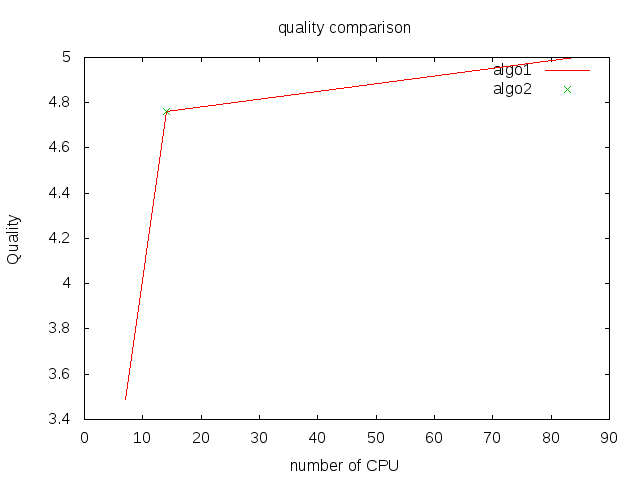
\includegraphics[width=0.8\linewidth]{Chapitre1/figures/comparison.png}
   \end{center}
   \caption[titre court pour la liste des figures]
   {\footnotesize Titre plus long avec des explications.}
   \label{fig:mafigure2}
\end{figure}


\subsection{Deuxième sous-section}

Morbi lorem. Etiam scelerisque rhoncus orci. Nunc elementum ante ac leo. Vestibulum venenatis dictum nunc. Donec turpis est, dictum nec, fringilla nec, cursus id, quam. In nibh orci, porttitor ut, rutrum id, faucibus vitae, leo. Donec ut wisi. Vivamus ornare, lorem quis tristique dapibus, nulla nisl nonummy libero, vitae luctus sem felis vel nisl. Suspendisse lectus lacus, ultricies vitae, feugiat et, hendrerit in, quam. Pellentesque porttitor enim at lectus. Praesent viverra laoreet velit. Mauris neque odio, ornare id, rhoncus non, sollicitudin sed, lectus. Phasellus et dolor. Aenean ullamcorper risus id libero. Pellentesque ac sem eget libero aliquam tincidunt. Suspendisse neque. Curabitur egestas neque ultrices nisl. Nulla bibendum augue et tellus. Duis ultrices convallis est.

Lorem ipsum dolor sit amet, consectetuer adipiscing elit. Maecenas fermentum, elit non lobortis cursus, orci velit suscipit est, id mollis turpis mi eget orci. Ut aliquam sollicitudin metus. Mauris at sapien sed sapien congue iaculis. Nulla lorem urna, bibendum id, laoreet iaculis, nonummy eget, massa. Phasellus ullamcorper commodo velit. Class aptent taciti sociosqu ad litora torquent per conubia nostra, per inceptos hymenaeos. Phasellus est. Maecenas felis augue, gravida quis, porta adipiscing, iaculis vitae, felis. Nullam ipsum. Nulla a sem ac leo fringilla mattis. Phasellus egestas augue in sem. Etiam ac enim non mauris ullamcorper scelerisque. In wisi leo, malesuada vulputate, tempor sit amet, facilisis vel, velit. Mauris massa est, sodales placerat, luctus id, hendrerit a, urna. Nullam eleifend pede eget odio. Duis non erat. Nullam pellentesque.

Lorem ipsum dolor sit amet, consectetuer adipiscing elit. Maecenas fermentum, elit non lobortis cursus, orci velit suscipit est, id mollis turpis mi eget orci. Ut aliquam sollicitudin metus. Mauris at sapien sed sapien congue iaculis. Nulla lorem urna, bibendum id, laoreet iaculis, nonummy eget, massa. Phasellus ullamcorper commodo velit. Class aptent taciti sociosqu ad litora torquent per conubia nostra, per inceptos hymenaeos. Phasellus est. Maecenas felis augue, gravida quis, porta adipiscing, iaculis vitae, felis. Nullam ipsum. Nulla a sem ac leo fringilla mattis. Phasellus egestas augue in sem. Etiam ac enim non mauris ullamcorper scelerisque. In wisi leo, malesuada vulputate, tempor sit amet, facilisis vel, velit. Mauris massa est, sodales placerat, luctus id, hendrerit a, urna. Nullam eleifend pede eget odio. Duis non erat. Nullam pellentesque.

Lorem ipsum dolor sit amet, consectetuer adipiscing elit. Maecenas fermentum, elit non lobortis cursus, orci velit suscipit est, id mollis turpis mi eget orci. Ut aliquam sollicitudin metus. Mauris at sapien sed sapien congue iaculis. Nulla lorem urna, bibendum id, laoreet iaculis, nonummy eget, massa. Phasellus ullamcorper commodo velit. Class aptent taciti sociosqu ad litora torquent per conubia nostra, per inceptos hymenaeos. Phasellus est. Maecenas felis augue, gravida quis, porta adipiscing, iaculis vitae, felis. Nullam ipsum. Nulla a sem ac leo fringilla mattis. Phasellus egestas augue in sem. Etiam ac enim non mauris ullamcorper scelerisque. In wisi leo, malesuada vulputate, tempor sit amet, facilisis vel, velit. Mauris massa est, sodales placerat, luctus id, hendrerit a, urna. Nullam eleifend pede eget odio. Duis non erat. Nullam pellentesque.

Lorem ipsum dolor sit amet, consectetuer adipiscing elit. Maecenas fermentum, elit non lobortis cursus, orci velit suscipit est, id mollis turpis mi eget orci. Ut aliquam sollicitudin metus. Mauris at sapien sed sapien congue iaculis. Nulla lorem urna, bibendum id, laoreet iaculis, nonummy eget, massa. Phasellus ullamcorper commodo velit. Class aptent taciti sociosqu ad litora torquent per conubia nostra, per inceptos hymenaeos. Phasellus est. Maecenas felis augue, gravida quis, porta adipiscing, iaculis vitae, felis. Nullam ipsum. Nulla a sem ac leo fringilla mattis. Phasellus egestas augue in sem. Etiam ac enim non mauris ullamcorper scelerisque. In wisi leo, malesuada vulputate, tempor sit amet, facilisis vel, velit. Mauris massa est, sodales placerat, luctus id, hendrerit a, urna. Nullam eleifend pede eget odio. Duis non erat. Nullam pellentesque.

Lorem ipsum dolor sit amet, «~consectetuer~» adipiscing elit. Maecenas fermentum, elit non lobortis cursus, orci velit suscipit est, id mollis turpis mi eget orci. Ut aliquam sollicitudin metus. Mauris at sapien sed sapien congue iaculis. Nulla lorem urna, bibendum id, laoreet iaculis, nonummy eget, massa. Phasellus ullamcorper commodo velit. Class aptent taciti sociosqu ad litora torquent per «~conubia nostra~», per inceptos hymenaeos. Phasellus est. Maecenas felis augue, gravida quis, porta adipiscing, iaculis vitae, felis. Nullam ipsum. Nulla a sem ac leo fringilla mattis. Phasellus egestas augue in sem. Etiam ac enim non mauris ullamcorper scelerisque. In wisi leo, malesuada vulputate, tempor sit amet, facilisis vel, velit. Mauris massa est, sodales placerat, luctus id, hendrerit a, urna. Nullam eleifend pede eget odio. Duis non erat. Nullam pellentesque.

Lorem ipsum dolor sit amet, «~consectetuer~» adipiscing elit. Maecenas fermentum, elit non lobortis cursus, orci velit suscipit est, id mollis turpis mi eget orci. Ut aliquam sollicitudin metus. Mauris at sapien sed sapien congue iaculis. Nulla lorem urna, bibendum id, laoreet iaculis, nonummy eget, massa. Phasellus ullamcorper commodo velit. Class aptent taciti sociosqu ad litora torquent per «~conubia nostra~», per inceptos hymenaeos. Phasellus est. Maecenas felis augue, gravida quis, porta adipiscing, iaculis vitae, felis. Nullam ipsum. Nulla a sem ac leo fringilla mattis. Phasellus egestas augue in sem. Etiam ac enim non mauris ullamcorper scelerisque. In wisi leo, malesuada vulputate, tempor sit amet, facilisis vel, velit. Mauris massa est, sodales placerat, luctus id, hendrerit a, urna. Nullam eleifend pede eget odio. Duis non erat. Nullam pellentesque.

Lorem ipsum dolor sit amet, «~consectetuer~» adipiscing elit. Maecenas fermentum, elit non lobortis cursus, orci velit suscipit est, id mollis turpis mi eget orci. Ut aliquam sollicitudin metus. Mauris at sapien sed sapien congue iaculis. Nulla lorem urna, bibendum id, laoreet iaculis, nonummy eget, massa. Phasellus ullamcorper commodo velit. Class aptent taciti sociosqu ad litora torquent per «~conubia nostra~», per inceptos hymenaeos. Phasellus est. Maecenas felis augue, gravida quis, porta adipiscing, iaculis vitae, felis. Nullam ipsum. Nulla a sem ac leo fringilla mattis. Phasellus egestas augue in sem. Etiam ac enim non mauris ullamcorper scelerisque. In wisi leo, malesuada vulputate, tempor sit amet, facilisis vel, velit. Mauris massa est, sodales placerat, luctus id, hendrerit a, urna. Nullam eleifend pede eget odio. Duis non erat. Nullam pellentesque.


\section{Conclusion du premier chapitre}


Lorem ipsum dolor sit amet, consectetuer adipiscing elit. Maecenas fermentum, elit non lobortis cursus, orci velit suscipit est, id mollis turpis mi eget orci. Ut aliquam sollicitudin metus. Mauris at sapien sed sapien congue iaculis. Nulla lorem urna, bibendum id, laoreet iaculis, nonummy eget, massa. Phasellus ullamcorper commodo velit. Class aptent taciti sociosqu ad litora torquent per conubia nostra, per inceptos hymenaeos. Phasellus est. Maecenas felis augue, gravida quis, porta adipiscing, iaculis vitae, felis. Nullam ipsum. Nulla a sem ac leo fringilla mattis. Phasellus egestas augue in sem. Etiam ac enim non mauris ullamcorper scelerisque. In wisi leo, malesuada vulputate, tempor sit amet, facilisis vel, velit. Mauris massa est, sodales placerat, luctus id, hendrerit a, urna. Nullam eleifend pede eget odio. Duis non erat. Nullam pellentesque.



\clearemptydoublepage

\chapter[ceci est un long titre]{Nom du chapitre 2}

Lorem ipsum dolor sit amet, «~consectetuer~» adipiscing elit. Maecenas fermentum, elit non lobortis cursus, orci velit suscipit est, id mollis turpis mi eget orci. Ut aliquam sollicitudin metus. Mauris at sapien sed sapien congue iaculis. Nulla lorem urna, bibendum id, laoreet iaculis, nonummy eget, massa. Phasellus ullamcorper commodo velit. Class aptent taciti sociosqu ad litora torquent per «~conubia nostra~», per inceptos hymenaeos. Phasellus est. Maecenas felis augue, gravida quis, porta adipiscing, iaculis vitae, felis. Nullam ipsum. Nulla a sem ac leo fringilla mattis. Phasellus egestas augue in sem. Etiam ac enim non mauris ullamcorper scelerisque. In wisi leo, malesuada vulputate, tempor sit amet, facilisis vel, velit. Mauris massa est, sodales placerat, luctus id, hendrerit a, urna. Nullam eleifend pede eget odio. Duis non erat. Nullam pellentesque\footcite[225]{Doule1887}.

\section{Première section du chapitre}

\subsection{Première sous-section}

Cras molestie. Curabitur id urna. Suspendisse tempor. Aliquam erat volutpat. Aliquam erat volutpat. Nam ultricies metus sit amet erat\footnote{Mauris neque odio, ornare id, rhoncus non, sollicitudin sed, lectus. Phasellus et dolor. Aenean ullamcorper risus id libero. Pellentesque ac sem eget libero aliquam tincidunt. Suspendisse neque.}. Suspendisse eget ipsum ut purus imperdiet suscipit. Mauris sed urna at diam volutpat placerat. Nulla vitae tortor. Nulla sed nisl.

Morbi lorem. Etiam scelerisque rhoncus orci. Nunc elementum ante ac leo. Vestibulum venenatis dictum nunc. Donec turpis est, dictum nec\footcite[228]{Drocher2006}, fringilla nec, cursus id, quam. In nibh orci, porttitor ut, rutrum id, faucibus vitae, leo. Donec ut wisi. Vivamus ornare, lorem quis tristique dapibus, nulla nisl nonummy libero, vitae luctus sem felis vel nisl. Suspendisse lectus lacus, ultricies vitae, feugiat et, hendrerit in, quam. Pellentesque porttitor enim at lectus. Praesent viverra laoreet velit. Mauris neque odio, ornare id, rhoncus non, sollicitudin sed, lectus. Phasellus et dolor. Aenean ullamcorper risus id libero. Pellentesque ac sem eget libero aliquam tincidunt. Suspendisse neque. Curabitur egestas neque ultrices nisl. Nulla bibendum augue et tellus. Duis ultrices convallis est.

Lorem ipsum dolor sit amet, consectetuer adipiscing elit. Maecenas fermentum, elit non lobortis cursus, orci velit suscipit est, id mollis turpis mi eget orci. Ut aliquam sollicitudin metus. Mauris at sapien sed sapien congue iaculis. Nulla lorem urna, bibendum id, laoreet iaculis, nonummy eget, massa. Phasellus ullamcorper commodo velit. Class aptent taciti sociosqu ad litora torquent per conubia nostra, per inceptos hymenaeos. Phasellus est. Maecenas felis augue, gravida quis, porta adipiscing, iaculis vitae, felis. Nullam ipsum. Nulla a sem ac leo fringilla mattis. Phasellus egestas augue in sem. Etiam ac enim non mauris ullamcorper scelerisque. In wisi leo, malesuada vulputate, tempor sit amet, facilisis vel, velit. Mauris massa est, sodales placerat, luctus id, hendrerit a, urna. Nullam eleifend pede eget odio. Duis non erat. Nullam pellentesque.


\subsection{Deuxième sous-section}

Morbi lorem. Etiam scelerisque rhoncus orci. Nunc elementum ante ac leo. Vestibulum venenatis dictum nunc. Donec turpis est, dictum nec, fringilla nec, cursus id, quam. In nibh orci, porttitor ut, rutrum id, faucibus vitae, leo. Donec ut wisi. Vivamus ornare, lorem quis tristique dapibus, nulla nisl nonummy libero, vitae luctus sem felis vel nisl. Suspendisse lectus lacus, ultricies vitae, feugiat et, hendrerit in, quam. Pellentesque porttitor enim at lectus. Praesent viverra laoreet velit. Mauris neque odio, ornare id, rhoncus non, sollicitudin sed, lectus. Phasellus et dolor. Aenean ullamcorper risus id libero. Pellentesque ac sem eget libero aliquam tincidunt. Suspendisse neque. Curabitur egestas neque ultrices nisl. Nulla bibendum augue et tellus. Duis ultrices convallis est.

Lorem ipsum dolor sit amet, consectetuer adipiscing elit. Maecenas fermentum, elit non lobortis cursus, orci velit suscipit est, id mollis turpis mi eget orci. Ut aliquam sollicitudin metus. Mauris at sapien sed sapien congue iaculis. Nulla lorem urna, bibendum id, laoreet iaculis, nonummy eget, massa. Phasellus ullamcorper commodo velit. Class aptent taciti sociosqu ad litora torquent per conubia nostra, per inceptos hymenaeos. Phasellus est. Maecenas felis augue, gravida quis, porta adipiscing, iaculis vitae, felis. Nullam ipsum. Nulla a sem ac leo fringilla mattis. Phasellus egestas augue in sem. Etiam ac enim non mauris ullamcorper scelerisque. In wisi leo, malesuada vulputate, tempor sit amet, facilisis vel, velit. Mauris massa est, sodales placerat, luctus id, hendrerit a, urna. Nullam eleifend pede eget odio. Duis non erat. Nullam pellentesque.

Lorem ipsum dolor sit amet, consectetuer adipiscing elit. Maecenas fermentum, elit non lobortis cursus, orci velit suscipit est, id mollis turpis mi eget orci. Ut aliquam sollicitudin metus. Mauris at sapien sed sapien congue iaculis. Nulla lorem urna, bibendum id, laoreet iaculis, nonummy eget, massa. Phasellus ullamcorper commodo velit. Class aptent taciti sociosqu ad litora torquent per conubia nostra, per inceptos hymenaeos. Phasellus est. Maecenas felis augue, gravida quis, porta adipiscing, iaculis vitae, felis. Nullam ipsum. Nulla a sem ac leo fringilla mattis. Phasellus egestas augue in sem. Etiam ac enim non mauris ullamcorper scelerisque. In wisi leo, malesuada vulputate, tempor sit amet, facilisis vel, velit. Mauris massa est, sodales placerat, luctus id, hendrerit a, urna. Nullam eleifend pede eget odio. Duis non erat. Nullam pellentesque.

\section{Conclusion du second chapitre}


Lorem ipsum dolor sit amet, consectetuer adipiscing elit. Maecenas fermentum, elit non lobortis cursus, orci velit suscipit est, id mollis turpis mi eget orci. Ut aliquam sollicitudin metus. Mauris at sapien sed sapien congue iaculis. Nulla lorem urna, bibendum id, laoreet iaculis, nonummy eget, massa. Phasellus ullamcorper commodo velit. Class aptent taciti sociosqu ad litora torquent per conubia nostra, per inceptos hymenaeos. Phasellus est. Maecenas felis augue, gravida quis, porta adipiscing, iaculis vitae, felis. Nullam ipsum. Nulla a sem ac leo fringilla mattis. Phasellus egestas augue in sem. Etiam ac enim non mauris ullamcorper scelerisque. In wisi leo, malesuada vulputate, tempor sit amet, facilisis vel, velit. Mauris massa est, sodales placerat, luctus id, hendrerit a, urna. Nullam eleifend pede eget odio. Duis non erat. Nullam pellentesque.

Lorem ipsum dolor sit amet, consectetuer adipiscing elit. Maecenas fermentum, elit non lobortis cursus, orci velit suscipit est, id mollis turpis mi eget orci. Ut aliquam sollicitudin metus. Mauris at sapien sed sapien congue iaculis. Nulla lorem urna, bibendum id, laoreet iaculis, nonummy eget, massa. Phasellus ullamcorper commodo velit. Class aptent taciti sociosqu ad litora torquent per conubia nostra, per inceptos hymenaeos. Phasellus est. Maecenas felis augue, gravida quis, porta adipiscing, iaculis vitae, felis. Nullam ipsum. Nulla a sem ac leo fringilla mattis. Phasellus egestas augue in sem. Etiam ac enim non mauris ullamcorper scelerisque. In wisi leo, malesuada vulputate, tempor sit amet, facilisis vel, velit. Mauris massa est, sodales placerat, luctus id, hendrerit a, urna. Nullam eleifend pede eget odio. Duis non erat. Nullam pellentesque.


\clearemptydoublepage
\backmatter
\chapter*{Conclusion}
\addcontentsline{toc}{chapter}{Conclusion}
\chaptermark{Conclusion}


Lorem ipsum dolor sit amet, «~consectetuer~» adipiscing elit. Maecenas fermentum, elit non lobortis cursus, orci velit suscipit est, id mollis turpis mi eget orci. Ut aliquam sollicitudin metus. Mauris at sapien sed sapien congue iaculis. Nulla lorem urna, bibendum id, laoreet iaculis, nonummy eget, massa. Phasellus ullamcorper commodo velit. Class aptent taciti sociosqu ad litora torquent per «~conubia nostra~», per inceptos hymenaeos. Phasellus est. Maecenas felis augue, gravida quis, porta adipiscing, iaculis vitae, felis. Nullam ipsum. Nulla a sem ac leo fringilla mattis. Phasellus egestas augue in sem. Etiam ac enim non mauris ullamcorper scelerisque. In wisi leo, malesuada vulputate, tempor sit amet, facilisis vel, velit. Mauris massa est, sodales placerat, luctus id, hendrerit a, urna. Nullam eleifend pede eget odio. Duis non erat. Nullam pellentesque.

\begin{verse}
Maître Corbeau, sur un arbre perché, \\
Tenait en son bec un fromage. \\
Maître Renard, par l'odeur alléché, \\
Lui tint à peu près ce langage : \\
«~Hé ! bonjour, Monsieur du Corbeau. \\
Que vous êtes joli ! que vous me semblez beau ! \\
Sans mentir, si votre ramage \\
Se rapporte à votre plumage, \\
Vous êtes le Phénix des hôtes de ces bois.~» \\
\end{verse}

Lorem ipsum dolor sit amet, consectetuer adipiscing elit. Maecenas fermentum, elit non lobortis cursus, orci velit suscipit est, id mollis turpis mi eget orci. Ut aliquam sollicitudin metus. Mauris at sapien sed sapien congue iaculis. Nulla lorem urna, bibendum id, laoreet iaculis, nonummy eget, massa\footcite[32]{Pierre1901}. Phasellus ullamcorper commodo velit. Class aptent taciti sociosqu ad litora torquent per conubia nostra, per inceptos hymenaeos. Phasellus est. Maecenas felis augue, gravida quis, porta adipiscing, iaculis vitae, felis. Nullam ipsum. Nulla a sem ac leo fringilla mattis. Phasellus egestas augue in sem. Etiam ac enim non mauris ullamcorper scelerisque. In wisi leo, malesuada vulputate, tempor sit amet, facilisis vel, velit. Mauris massa est, sodales placerat, luctus id, hendrerit a, urna. Nullam eleifend pede eget odio. Duis non erat. Nullam pellentesque. 

\section*{Première section de l'intro}
\addcontentsline{toc}{section}{Première section de l'intro}

Lorem ipsum dolor sit amet, «~consectetuer~» adipiscing elit. Maecenas fermentum, elit non lobortis cursus, orci velit suscipit est, id mollis turpis mi eget orci. Ut aliquam sollicitudin metus. Mauris at sapien sed sapien congue iaculis. Nulla lorem urna, bibendum id, laoreet iaculis, nonummy eget, massa. Phasellus ullamcorper commodo velit. Class aptent taciti sociosqu ad litora torquent per «~conubia nostra~», per inceptos hymenaeos. Phasellus est. Maecenas felis augue, gravida quis, porta adipiscing, iaculis vitae, felis. Nullam ipsum. Nulla a sem ac leo fringilla mattis. Phasellus egestas augue in sem. Etiam ac enim non mauris ullamcorper scelerisque. In wisi leo, malesuada vulputate, tempor sit amet, facilisis vel, velit. Mauris massa est, sodales placerat, luctus id, hendrerit a, urna. Nullam eleifend pede eget odio. Duis non erat. Nullam pellentesque.

\textbf{Une boite magique : }

\boitemagique{Titre de la boite}{
Praesent placerat, ante at venenatis pretium, diam turpis faucibus arcu, nec vehicula quam lorem ut leo. Sed facilisis, augue in pharetra dapibus, ligula justo accumsan massa, eu suscipit felis ipsum eget enim.
}

Laoreet iaculis, nonummy eget, massa. Phasellus ullamcorper commodo velit. Class aptent taciti sociosqu ad litora torquent per «~conubia nostra~», per inceptos hymenaeos. Phasellus est. Maecenas felis augue, gravida quis, porta adipiscing, iaculis vitae, felis. Nullam ipsum. Nulla a sem ac leo fringilla mattis. Phasellus egestas augue in sem. Etiam ac enim non mauris ullamcorper scelerisque. In wisi leo, malesuada vulputate, tempor sit amet, facilisis vel, velit. Mauris massa est, sodales placerat, luctus id, hendrerit a, urna. Nullam eleifend pede eget odio. Duis non erat. Nullam pellentesque.

\textbf{Une boite simple : }
\boitesimple{Mauris lorem quam, tristique sollicitudin egestas sed, sodales vel leo. In hac habitasse platea dictumst. Lorem ipsum dolor sit amet, consectetur adipiscing elit. Sed sed lorem lacus, at venenatis elit. Pellentesque nisl arcu, blandit ac eleifend non, sodales a quam.}

Laoreet iaculis, nonummy eget, massa. Phasellus ullamcorper commodo velit. Class aptent taciti sociosqu ad litora torquent per «~conubia nostra~», per inceptos hymenaeos. Phasellus est. Maecenas felis augue, gravida quis, porta adipiscing, iaculis vitae, felis. Nullam ipsum. Nulla a sem ac leo fringilla mattis. Phasellus egestas augue in sem. Etiam ac enim non mauris ullamcorper scelerisque. In wisi leo, malesuada vulputate, tempor sit amet, facilisis vel, velit. Mauris massa est, sodales placerat, luctus id, hendrerit a, urna. Nullam eleifend pede eget odio. Duis non erat. Nullam pellentesque.




% Chapitre pour la bibliographie
% Bibliography chapter
\clearemptydoublepage
\phantomsection % To have a correct link in the table of contents
\addcontentsline{toc}{chapter}{Bibliography}
\chapter{La biblio devrait être ici}

% nocite: Pour citer la totalit\'{e} des r\'{e}f\'{e}rences contenues dans le fichier biblio
% nocite: In order to cite all the references included biblio
\nocite{*}
\printbibliography[heading=primary,keyword=primary]
\newpage
\nocite{*}
\printbibliography[heading=secondary,keyword=secondary]

\clearemptydoublepage
% Pour avoir la quatrième de couverture sur une page paire
% To have the back cover on an even page
\cleartoevenpage[\thispagestyle{empty}]
\markboth{}{}
% Plus petite marge du bas pour la quatrième de couverture
% Shorter bottom margin for the back cover
\newgeometry{inner=30mm,outer=20mm,top=40mm,bottom=20mm}

%insertion de l'image de fond du dos (resume)
%background image for resume (back)
\backcoverheader

% Switch font style to back cover style
\selectfontbackcover{ % Font style change is limited to this page using braces, just in case

\titleFR{titre (en fran\c cais)..............}

\keywordsFR{de 3 \`{a} 6 mots clefs}

\abstractFR{Eius populus ab incunabulis primis ad usque pueritiae tempus extremum, quod annis circumcluditur fere trecentis, circummurana pertulit bella, deinde aetatem ingressus adultam post multiplices bellorum aerumnas Alpes transcendit et fretum, in iuvenem erectus et virum ex omni plaga quam orbis ambit inmensus, reportavit laureas et triumphos, iamque vergens in senium et nomine solo aliquotiens vincens ad tranquilliora vitae discessit.
Hoc inmaturo interitu ipse quoque sui pertaesus excessit e vita aetatis nono anno atque vicensimo cum quadriennio imperasset. natus apud Tuscos in Massa Veternensi, patre Constantio Constantini fratre imperatoris, matreque Galla.
Thalassius vero ea tempestate praefectus praetorio praesens ipse quoque adrogantis ingenii, considerans incitationem eius ad multorum augeri discrimina, non maturitate vel consiliis mitigabat, ut aliquotiens celsae potestates iras principum molliverunt, sed adversando iurgandoque cum parum congrueret, eum ad rabiem potius evibrabat, Augustum actus eius exaggerando creberrime
docens, idque, incertum qua mente, ne lateret adfectans. quibus mox Caesar acrius efferatus, velut contumaciae quoddam vexillum altius erigens, sine respectu salutis alienae vel suae ad vertenda opposita instar rapidi fluminis irrevocabili impetu ferebatur.
Hae duae provinciae bello quondam piratico catervis mixtae praedonum.}



\titleEN{titre (en anglais)..............}

\keywordsEN{de 3 \`{a} 6 mots clefs}

\abstractEN{Eius populus ab incunabulis primis ad usque pueritiae tempus extremum, quod annis circumcluditur fere trecentis, circummurana pertulit bella, deinde aetatem ingressus adultam post multiplices bellorum aerumnas Alpes transcendit et fretum, in iuvenem erectus et virum ex omni plaga quam orbis ambit inmensus, reportavit laureas et triumphos, iamque vergens in senium et nomine solo aliquotiens vincens ad tranquilliora vitae discessit.
Hoc inmaturo interitu ipse quoque sui pertaesus excessit e vita aetatis nono anno atque vicensimo cum quadriennio imperasset. natus apud Tuscos in Massa Veternensi, patre Constantio Constantini fratre imperatoris, matreque Galla.
Thalassius vero ea tempestate praefectus praetorio praesens ipse quoque adrogantis ingenii, considerans incitationem eius ad multorum augeri discrimina, non maturitate vel consiliis mitigabat, ut aliquotiens celsae potestates iras principum molliverunt, sed adversando iurgandoque cum parum congrueret, eum ad rabiem potius evibrabat, Augustum actus eius exaggerando creberrime
docens, idque, incertum qua mente, ne lateret adfectans. quibus mox Caesar acrius efferatus, velut contumaciae quoddam vexillum altius erigens, sine respectu salutis alienae vel suae ad vertenda opposita instar rapidi fluminis irrevocabili impetu ferebatur.
Hae duae provinciae bello quondam piratico catervis mixtae praedonum.}

}

% Rétablit les marges d'origines
% Restore original margin settings
\restoregeometry


\end{document}
